\documentclass[CHICAGO]{USG}
\usepackage{tikz}
\usetikzlibrary{arrows.meta,fit,positioning,shapes.geometric}
\usepackage{booktabs}
\usepackage{multirow}
\usepackage{array}
\usepackage{xcolor}
\graphicspath{{./images/}}

\makeatletter
\def\@@articletype{%
  \rule[-4\@p@t]{4\@p@t}{15\@p@t}%
  \hskip -0\@p@t%
  {\arttypefont\bf\uppercase{\letterspace to 1.15\naturalwidth{\@articletype}}}%
}%
\renewcommand{\@@address}[2][]{\def\temp{#1}%
\g@addto@macro\jmkaddress{\hsize=\textwidth%
\def\baselinestretch{1}%
\stepcounter{affn}%
\xdef\@currentlabel{\theaffn}%
\jmkLabel{#1}%
\addressfont\ifx#1\empty\else\@hangfrom{\textsuperscript{\smash{\theaffn}}}\fi%
#2%
}}%
\makeatother
\newcommand{\TBD}[1]{\textcolor{red}{[TBD: #1]}}


\articletype{ORIGINAL ARTICLE}
\journal{Expert Systems}
\volume{0}
\copyyear{2026}
\startpage{1}
\articledoi{10.1002/exsy.00000}
\received{00}
\revised{00}
\accepted{00}

\begin{document}
\title{Diagnosing and Correcting Score Fusion in a Cold-Start Volunteering Recommender: A Single-Profile Case Study with External Validation}
\transtitle{Diagnosing and Correcting Score Fusion in a Cold-Start Volunteering Recommender: A Single-Profile Case Study with External Validation}

\author[1]{Ayla Kayaba\c{s}}[https://orcid.org/0000-0002-6584-5130]
\author[1]{Aziz Muammer \c{C}etiner}[https://orcid.org/0009-0004-7159-9265]

\authormark{KAYABA\c{S} \textsc{et al.}}
\titlemark{Diagnosing score fusion in a volunteering recommender}

\address{\orgdiv{Department of Computer Engineering, }\orgname{K{\i}r\c{s}ehir Ahi Evran University, }%
\orgaddress{\state{K{\i}r\c{s}ehir, }\country{T\"urkiye}}}

\corres{Ayla Kayaba\c{s} (\email{ayla.kayabas@ahievran.edu.tr})}

\fundingInfo{Scientific and Technological Research Council of T\"urkiye (T\"UB\.{I}TAK), 2209-A University Students Research Projects Support Program, Grant/Award Number: 1919B012503272.}

\keywords{cold start | content-based recommendation | error analysis | external validation | sentence embeddings | volunteering recommendation}

\abstract[ABSTRACT]{Volunteering listings on the European Youth Portal close at a deadline, so a recommender must rank them from content alone. We built a ranker that fuses three inspectable scores computed from a CV, a motivation letter, and the listing text, and applied it to 939 listings and one candidate. Its skill-matching score lay between 99.39 and 99.87 for every listing with skills. The diagnosis traced this to two mechanisms: one coordinate carried a median 97\% of the squared norm of the XLM-RoBERTa skill vectors and compressed all cosines toward one, and the encoder did not separate related from unrelated skills, with a ROC-AUC of 0.627 on 4{,}000 ESCO skill pairs that was unchanged without that coordinate. We corrected six faults, selected a sentence encoder on the ESCO pairs (AUC 0.976), froze three versions of the ranker, and described it with label-free diagnostics. On TalentCLEF 2026 Task A, the corrected matching score exceeded the original on all four metrics, significantly only for Recall@100 (+0.249, Holm-adjusted $p=0.016$); no difference from a dense retriever was detected, and it was below BM25 on MAP and Recall@100. The study uses one candidate profile, and the volunteering recommendations were not validated against relevance labels.}

\maketitle

\section{Introduction}
\label{sec:introduction}

The European Youth Portal publishes the volunteering listings of the European Solidarity Corps, a European Union programme that funds volunteering placements for young people, and each listing remains open only until its application deadline~\citep{eyp}. A listing therefore often closes before it accumulates clicks or ratings, and a candidate who visits the portal for the first time has no interaction history either. This is the cold-start problem of collaborative filtering: a new item or a new user without ratings cannot be placed reliably in a ranking that depends on ratings~\citep{lika2014}. A ranker for such listings has to rely on content that exists before any interaction, namely the listing text and the documents that the candidate submits, such as a CV and a motivation letter.

A ranker of this kind can expose its reasoning as a small number of scores, for example how well the CV covers the skills that a listing names, how closely the letter relates to the listing, and whether the CV gives evidence for the listed skills. Scores that a user can inspect and weight respond to concerns about the opacity of recommender systems~\citep{ruohonen2024} and to the mechanisms for user control reviewed by \citet{jannach2017}. Exposed scores are only useful, however, if each of them measures what its name suggests and varies enough to influence the order.

We built such a ranker for one candidate and a snapshot of 939 listings, and its scores did not behave as intended. The matching score lay between 99.39 and 99.87 for every listing with skills, the letter score was nearly constant and depended on the length of the description, and standardization before fusion turned these narrow ranges into the main influence on the order. %
Because the snapshot has no relevance labels, the fused list looked plausible and the faults were not visible in it. This paper reports how the faults were diagnosed, how they were corrected, and what the correction changes, and it measures the cost of the main fault on an external dataset with relevance labels. It addresses three research questions:
\begin{itemize}
\item \textbf{RQ1.} What do the scores of the original ranker measure, and why did they fail to separate listings?
\item \textbf{RQ2.} What does the correction change in the scores and in the ranking of the volunteering listings?
\item \textbf{RQ3.} What does the diagnosed fault of the matching score cost on labeled data, and how much of that cost does the correction recover?
\end{itemize}

The contributions are as follows:
\begin{enumerate}
\item A diagnosis of six faults in a three-score ranker applied to a real listing pool, including a dominant coordinate in the skill vectors and an encoding that does not separate related from unrelated skills (Section~\ref{sec:diagnosis}, Table~\ref{tab:diagnosis}).
\item A corrected ranker whose encoder and thresholds are selected on public skill relations from ESCO, released in three versions that record which decisions were made before and after which outputs were seen (Sections~\ref{sec:corrected} and~\ref{sec:res-encoder}).
\item Label-free diagnostics of the corrected ranker on the volunteering snapshot: the spread of each score, its dependence on description length, the agreement with lexical and dense baselines, and the diversity of the leading listings relative to random lists (Section~\ref{sec:res-labelfree}).
\item An external validation on TalentCLEF 2026 Task A that quantifies the cost of the diagnosed fault and the part of it that the correction recovers, and that places the corrected matching score relative to BM25 and a dense retriever (Section~\ref{sec:res-talentclef}).
\item Three checks to run before score fusion, namely the spread of each component over the pool, its correlation with a confounder such as description length, and the ability of the encoder to separate labeled related and unrelated pairs, each of which would have exposed a fault of the original ranker (Section~\ref{sec:disc-lessons}).
\item Code, configurations, and outputs without personal data, frozen by git tags, from which every reported value can be recomputed (Data Availability Statement).
\end{enumerate}

Section~\ref{sec:related} reviews related work. Section~\ref{sec:system} describes the data and the original ranker, Section~\ref{sec:diagnosis} the diagnosis, Section~\ref{sec:corrected} the corrected ranker, and Section~\ref{sec:protocol} the evaluation protocol. Section~\ref{sec:results} reports the results, Section~\ref{sec:discussion} discusses them, Section~\ref{sec:limitations} states the limitations, and Section~\ref{sec:conclusion} answers the research questions.

\section{Related Work}
\label{sec:related}

\subsection{Cold Start and Content-Based Ranking}
\citet{lika2014} review collaborative filtering under cold start and use demographic attributes of new users to find similar users when ratings are missing. \citet{burke2002} classifies hybrid recommenders that combine collaborative and content-based components, for example through a weighted sum of their scores. Content-based components can score a new item from its description alone, which makes them applicable to listings that close before they are rated.

\subsection{Job and Skill Matching}
Matching people to opportunities is studied mainly for jobs. \citet{deruijt2021review} review a decade of job recommender research and stress that job matching is time-dependent and two-sided and that the available data shape the choice of method. Skills are a common intermediate representation: SkillNER extracts skill phrases from text by matching them against a skill database~\citep{skillner}, ESCO provides a multilingual European classification of skills and occupations with explicit relations between skills~\citep{esco}, and JobBERT learns representations of job titles from the skills extracted from vacancies~\citep{decorte2021jobbert}. TalentCLEF 2026 provides shared benchmarks for this area, including a task in which CVs are ranked for job postings~\citep{talentclef2026,gasco2026overview}. Volunteering listings differ from job postings in that they are written by many small hosts, partly in languages other than English, and are not labeled for relevance; the present work uses the job-matching benchmark only to validate the matching score.

\subsection{Sentence Embeddings and the Geometry of Contextual Representations}
Encoders trained for sentence similarity, such as Sentence-BERT~\citep{reimers2019} and its multilingual variants obtained by knowledge distillation~\citep{reimers2020}, as well as LaBSE~\citep{feng2022} and multilingual E5~\citep{wang2024me5}, produce vectors whose cosine similarity is meant to reflect semantic relatedness. Masked language models such as XLM-RoBERTa~\citep{conneau2020} are not trained for this purpose. \citet{ethayarajh2019} reports that their contextual representations occupy a narrow cone, so that the cosine between unrelated words is high. \citet{timkey2021} show that cosine similarity and Euclidean distance in such models are dominated by a small number of rogue dimensions, often one to three, and propose postprocessing such as standardization. \citet{kovaleva2021} find high-magnitude outlier dimensions in the LayerNorm parameters of BERT and related encoders whose removal degrades performance. The diagnosis in Section~\ref{sec:diagnosis} observes a dominant coordinate of this kind in practice and measures how much it explains.

\subsection{Trust and Text-Quality Signals}
\citet{massa2004} replace the similarity weight of collaborative filtering with a weight derived from explicit trust statements, and \citet{moradi2015} estimate the reliability of predicted ratings in a trust-aware recommender; both operate on a graph of users. For text written by one candidate, natural language inference (NLI) models classify whether a premise entails, contradicts, or is neutral toward a hypothesis and are commonly trained on corpora such as MultiNLI~\citep{williams2018}. Detectors of machine-generated text, such as the RoBERTa-based detector released with GPT-2~\citep{solaiman2019}, estimate the probability that a text was produced by a language model, but they misclassify a large share of essays by non-native English writers as machine-generated~\citep{liang2023}.

\subsection{Fusion, Diversity, and User Control}
A weighted hybrid computes a linear combination of component scores~\citep{burke2002,alshamlan2023}; such a combination assumes that the components vary on comparable scales. Maximal marginal relevance (MMR) re-ranks a list by trading the relevance of each next item against its similarity to the items already selected~\citep{carbonell1998}, and intra-list similarity measures how similar the items of a list are~\citep{ziegler2005}; both depend on a similarity measure that separates related from unrelated items. \citet{jannach2017} review mechanisms that let users control recommendations, and \citet{parra2015} evaluated a hybrid recommender whose fusion weights were exposed as interactive controls in a study with 40 participants. \citet{ruohonen2024} report predominantly negative views of recommender systems, including perceptions of opacity, in responses to a European Union consultation.

\subsection{Reproducibility and Auditing of Recommender Systems}
\citet{ferraridacrema2019} examined 18 top-$n$ recommendation algorithms from recent conferences, could reproduce 7 of them with reasonable effort, and found that 6 of these were often outperformed by comparably simple heuristic methods, such as nearest-neighbor techniques. They point to the reproducibility of results and the choice of baselines as methodological problems. The present paper applies a similar audit to a single prototype: it recomputes every score from stored outputs, traces each fault to the code, and evaluates the corrected system against simple baselines on labeled data.

\section{System and Data}
\label{sec:system}

\subsection{Study Design}
\label{sec:design}
The study has three steps. First, it diagnoses why the scores of a content-based ranker that was applied to one volunteering snapshot did not separate listings (Section~\ref{sec:diagnosis}). Second, it corrects each diagnosed fault and freezes the corrected ranker in three versions (Section~\ref{sec:corrected}). Third, it evaluates the correction in two ways (Section~\ref{sec:protocol}): with label-free diagnostics on the volunteering snapshot, for which no relevance labels exist, and with relevance labels on an external job-matching dataset. Fig.~\ref{fig:pipeline} compares the original and the corrected ranker. Throughout the paper, the \emph{original run} denotes the ranking that the first version of the system produced for the snapshot; its scores were recomputed from the stored output files.

\begin{figure*}[!t]
\centering
\resizebox{\textwidth}{!}{%
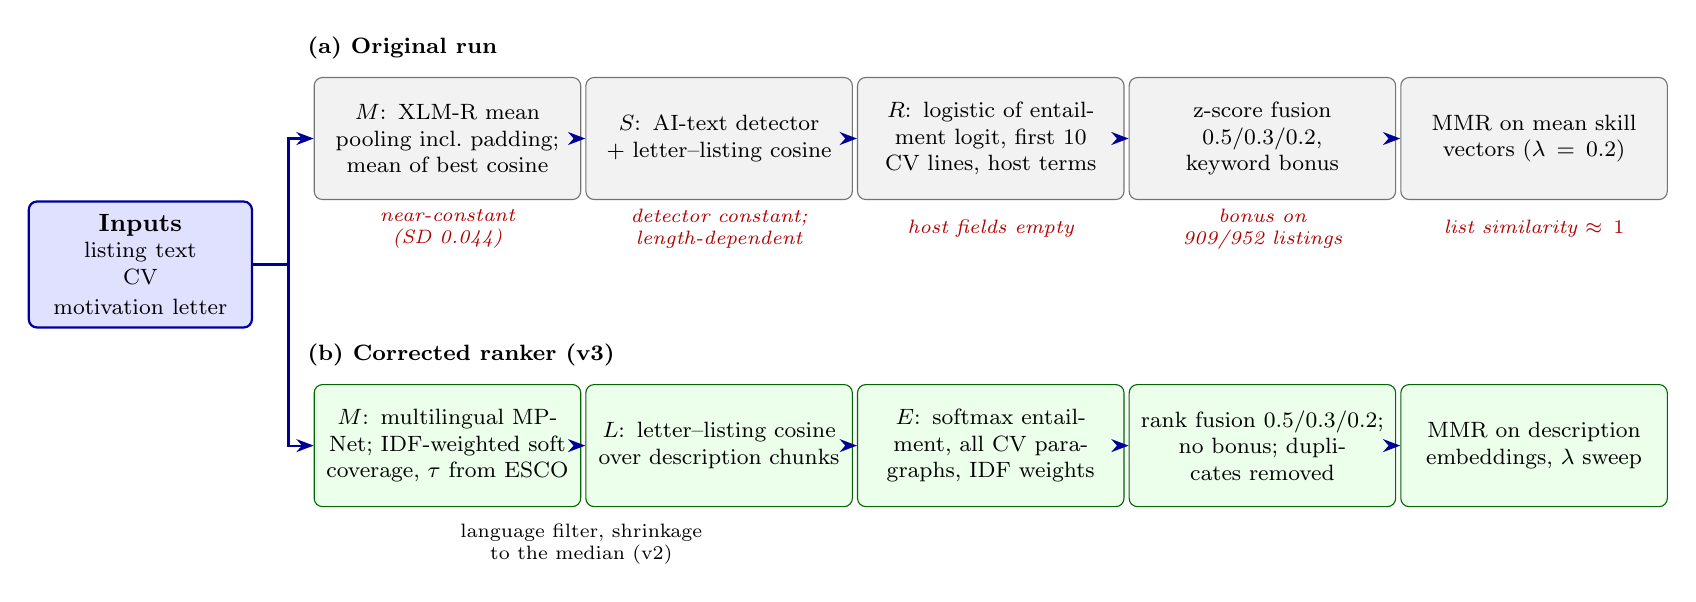
\begin{tikzpicture}[
  font=\small,
  inbox/.style={draw=blue!60!black, fill=blue!12, rounded corners=3pt, align=center, line width=0.8pt, text width=2.6cm, minimum height=1.6cm},
  old/.style={draw=black!55, fill=black!5, rounded corners=3pt, align=center, text width=3.15cm, minimum height=1.55cm, font=\footnotesize},
  new/.style={draw=green!40!black, fill=green!8, rounded corners=3pt, align=center, text width=3.15cm, minimum height=1.55cm, font=\footnotesize},
  bad/.style={font=\scriptsize\itshape, text=red!70!black, align=center, text width=3.15cm},
  arr/.style={-{Stealth[length=2.2mm]}, line width=0.8pt, blue!60!black},
  lbl/.style={font=\footnotesize\bfseries, anchor=west}
]
\node[inbox] (in) at (0,0) {\textbf{Inputs}\\\footnotesize listing text\\\footnotesize CV\\\footnotesize motivation letter};
\node[lbl] at (2.0,2.75) {(a) Original run};
\node[old] (oM) at (3.9,1.6) {$M$: XLM-R mean pooling incl.\ padding; mean of best cosine};
\node[old] (oS) at (7.35,1.6) {$S$: AI-text detector $+$ letter--listing cosine};
\node[old] (oR) at (10.8,1.6) {$R$: logistic of entailment logit, first 10 CV lines, host terms};
\node[old] (oF) at (14.25,1.6) {z-score fusion $0.5/0.3/0.2$, keyword bonus};
\node[old] (oX) at (17.7,1.6) {MMR on mean skill vectors ($\lambda=0.2$)};
\node[bad] at (3.9,0.45) {near-constant (SD 0.044)};
\node[bad] at (7.35,0.45) {detector constant; length-dependent};
\node[bad] at (10.8,0.45) {host fields empty};
\node[bad] at (14.25,0.45) {bonus on 909/952 listings};
\node[bad] at (17.7,0.45) {list similarity $\approx 1$};
\node[lbl] at (2.0,-1.15) {(b) Corrected ranker (v3)};
\node[new] (nM) at (3.9,-2.3) {$M$: multilingual MPNet; IDF-weighted soft coverage, $\tau$ from ESCO};
\node[new] (nL) at (7.35,-2.3) {$L$: letter--listing cosine over description chunks};
\node[new] (nE) at (10.8,-2.3) {$E$: softmax entailment, all CV paragraphs, IDF weights};
\node[new] (nF) at (14.25,-2.3) {rank fusion $0.5/0.3/0.2$; no bonus; duplicates removed};
\node[new] (nX) at (17.7,-2.3) {MMR on description embeddings, $\lambda$ sweep};
\node[font=\scriptsize, align=center, text width=3.15cm] at (5.6,-3.55) {language filter, shrinkage to the median (v2)};
\draw[arr] (in.east) -- ++(0.45,0) |- (oM.west);
\draw[arr] (in.east) -- ++(0.45,0) |- (nM.west);
\foreach \a/\b in {oM/oS,oS/oR,oR/oF,oF/oX,nM/nL,nL/nE,nE/nF,nF/nX} \draw[arr] (\a) -- (\b);
\end{tikzpicture}}
\caption{Original run and corrected ranker. (a) The original run computes a matching score $M$, a sincerity score $S$, and a reliability score $R$ for each listing, standardizes them, adds a keyword bonus, and re-ranks the first positions with maximal marginal relevance (MMR); the red notes give the fault that Section~\ref{sec:diagnosis} diagnoses for each step. (b) The corrected ranker replaces $S$ by the letter--listing relevance $L$ and $R$ by the CV evidence $E$, uses a sentence encoder selected on public skill relations, fuses percentile ranks, and reports MMR for several values of $\lambda$. The scores in both rows are computed separately for each listing.}
\label{fig:pipeline}
\end{figure*}

\subsection{Data}
\label{sec:data}
The listing pool is a snapshot of 952 records of open volunteering listings collected from the European Youth Portal~\citep{eyp} in December 2025. %
Thirteen records repeat another record with the same link, so the snapshot contains 939 distinct listings; the corrected ranker scores these 939 listings. %
For each listing, the stored output contains the link, the full description, and the skill phrases that SkillNER~\citep{skillner} extracted from the description with the spaCy model \texttt{en\_core\_web\_lg}. %
Seventy-two of the 939 descriptions are not in English, as judged by the spaCy stopword list that covers most of their words. %
Twenty-one listings have no extracted skill phrase, and 90 listings share their description with at least one other listing. %
A separate detailed scrape of 1{,}242 listings contains host attributes (organization name, address, website, and a verified flag); the first three are empty and the flag is false on every row. Of the 952 records, 622 appear in that scrape, and 564 of these 622 have no recorded application deadline. %

The candidate side consists of the Europass CV and the motivation letter of one of the authors, used with that author's consent. The CV has 32 paragraphs, where a paragraph is a line with more than 20 characters, and SkillNER extracts 49 skill phrases from it after cleaning. %
The motivation letter consists of four sentences about the author's volunteering abroad. %
No other person's data were used, and no relevance label was collected for any listing.

\subsection{Original Ranker}
\label{sec:original}
The original run computed three scores for each listing $p$ and the candidate $u$.

\emph{Matching score.} Let $\mathbf{p}_1,\ldots,\mathbf{p}_m$ be the vectors of the skills extracted from listing $p$ and $\mathbf{u}_1,\ldots,\mathbf{u}_n$ those of the CV skills. Each skill phrase was encoded with XLM-RoBERTa (\texttt{xlm-roberta-base})~\citep{conneau2020} by averaging the last hidden layer over all positions of the padded batch, and
\begin{equation}
M_{\mathrm{old}}(u,p) = \frac{100}{m}\sum_{j=1}^{m}\max_{k}\cos(\mathbf{p}_j,\mathbf{u}_k).
\label{eq:mold}
\end{equation}
A listing without skills received $M_{\mathrm{old}}=0$.

\emph{Sincerity score.} A RoBERTa classifier for text generated by GPT-2 (\texttt{roberta-base-openai-detector})~\citep{solaiman2019} assigned the letter a probability $P_{\mathrm{AI}}$, and the score combined its complement with the cosine between the mean-pooled XLM-RoBERTa embeddings of the letter and the description: $S(p) = 0.4\cdot100(1-P_{\mathrm{AI}}) + 0.6\,S_{\mathrm{context}}(p)$, with $S_{\mathrm{context}}(p)=100\cos(\mathbf{v}_{\mathrm{letter}},\mathbf{v}_p)$. %

\emph{Reliability score.} For each listing skill $s$, an NLI cross-encoder (\texttt{cross-encoder/nli-distilroberta-base}) scored the hypothesis ``I have the skill of $s$.'' against each of the first ten CV paragraphs. The skill score was the logistic function of the largest entailment logit times 100, the listing score was the mean over its skills, and host bonuses and penalties for missing host attributes were added. %

\emph{Fusion and re-ranking.} Each score $x$ was standardized over the pool as $\tilde{x}=\min(100,\max(0,50+20(x-\mu_x)/\sigma_x))$ and fused as $F=0.5\tilde{M}+0.3\tilde{S}+0.2\tilde{R}$. A listing whose description contained one of the substrings \texttt{culture}, \texttt{art}, \texttt{heritage}, or \texttt{diversity} received 5 additional points, giving the adjusted score $A$. Finally, MMR~\citep{carbonell1998} re-selected the first 20 positions with $\lambda=0.2$, using the cosine between the mean skill vectors of two listings as their similarity. %

\section{Diagnosis}
\label{sec:diagnosis}

The diagnosis recomputed every score of the original run from the stored outputs and the source code, and it inspected the intermediate values (vectors, logits, and per-listing components) wherever a score showed little variation. Six faults were found.

\emph{D1: the matching score was nearly constant.} Over the 898 listings that keep at least one skill after the language filter of Section~\ref{sec:skills}, $M_{\mathrm{old}}$ ranged from 99.39 to 99.87, with a standard deviation of 0.044. %
Two properties of the encoding contributed to this. First, the unnormalized vectors had one dominant coordinate. The original run stored its skill vectors in printed form, which is complete only for listings with a single skill; in all 54 complete non-zero vectors, the largest absolute coordinate was dimension 741, with a median value of 18.32 (5th--95th percentile 18.17--18.40), whereas the median absolute value of the other 767 coordinates was 0.038. %
To avoid relying on 54 vectors, 2{,}004 skills of 223 randomly drawn listings were encoded again exactly as in the original run; the re-encoded values agreed with all values printed for 221 of these listings (median absolute difference $8\times10^{-8}$), and dimension 741 was again the largest coordinate in every vector, with a median value of 18.28. %
This coordinate carried 97\% of the squared norm, so the cosine between two arbitrary skill vectors was close to one: for random pairs of re-encoded skills, the median cosine was 0.995, and 0.833 after that coordinate was removed. %
Outlier dimensions of this kind have been reported for BERT-type models, where a few coordinates dominate cosine similarity~\citep{kovaleva2021,timkey2021}, and the observation is consistent with the anisotropy of contextual embeddings~\citep{ethayarajh2019}. Removing the coordinate widened the range of cosines but did not make related skills more similar than unrelated ones: on the ESCO pairs of Section~\ref{sec:encoder}, the ROC-AUC of the original encoding was 0.627 with all coordinates and 0.626 without dimension 741. %
Second, the mean over all positions included the padding positions of the batch, so the vector of a short skill phrase depended on the length of the longest phrase in the same batch. Masking the padding raised the AUC on the ESCO pairs to 0.751, which is still well below that of encoders trained for sentence similarity (Section~\ref{sec:res-encoder}). %
Because Eq.~\eqref{eq:mold} keeps the best match for each listing skill, almost every listing skill found a CV skill with a cosine close to one, and the remaining differences did not reflect relatedness.

\emph{D2: the sincerity score measured the letter once and the description length otherwise.} The detector assigned the letter $P_{\mathrm{AI}}=0.9996$, so its component had the same value for every listing; such detectors are known to misclassify text by non-native English writers~\citep{liang2023}. %
The context component had a mean of 99.72 and a standard deviation of 0.098, and its Spearman correlation with the length of the description in characters was $-0.55$. %
After standardization, a difference of 0.001 in cosine therefore moved $\tilde{S}$ by about 20 points.

\emph{D3: the reliability score used a partial NLI output, part of the CV, and empty host data.} The logistic function of the entailment logit ignores the contradiction and neutral logits, and the score used only the first 10 of the 32 CV paragraphs. %
The host adjustment had the same value for every listing that appears in the detailed scrape, because the host attributes are empty there (Section~\ref{sec:data}).

\emph{D4: the keyword bonus applied to almost every listing.} The substring test matched 909 of the 952 descriptions, for example because \texttt{art} occurs in ``participant'' and ``start''. %

\emph{D5: duplicated records.} The 13 repeated records were scored and ranked as separate listings. %

\emph{D6: standardization moved the decision to the other components, and MMR could not separate listings.} Because $\tilde{M}$ hardly varied, the order of the original run followed $\tilde{S}$ and $\tilde{R}$: over the 931 records with extracted skills, the Spearman correlation of $A$ was 0.06 with the raw matching score, 0.71 with $\tilde{S}$, and 0.33 with $\tilde{R}$. %
The mean pairwise cosine of the mean skill vectors of the first five listings was 0.9972, so the diversity term of MMR varied too little to change the selection. %

\section{Corrected Ranker}
\label{sec:corrected}

Each correction addresses one fault, and Table~\ref{tab:diagnosis} summarizes them with their measured effects. The corrected ranker keeps the three-score design and the original weights.

\subsection{Encoder Selection}
\label{sec:encoder}
The encoders of the corrected ranker were selected by a rule fixed in advance: the candidate with the highest ROC-AUC for separating related from unrelated skill pairs by cosine similarity, with ties broken by the larger difference between the median cosines of the two groups. The five candidates were XLM-RoBERTa with and without a padding mask, the multilingual paraphrase model \texttt{paraphrase-multilingual-mpnet-base-v2}~\citep{reimers2020}, LaBSE~\citep{feng2022}, and \texttt{multilingual-e5-base}~\citep{wang2024me5}. %
The two thresholds of the matching score (Section~\ref{sec:matching}) were set to the median cosine of the unrelated pairs ($\tau_{\mathrm{low}}$) and of the related pairs ($\tau_{\mathrm{high}}$) under the selected encoder. %

The rule was applied to two sets of pairs. The first set consisted of 100 pairs (50 related) written by hand; it was drafted with an AI assistant and checked by the authors (Section~\ref{sec:ai}). %
Because the multilingual MPNet model separated these pairs perfectly, the set could not distinguish between strong encoders; moreover, the pairs were drafted with the same AI assistant that helped implement the system, so they were not independent of it. It was therefore replaced by 4{,}000 pairs derived automatically from the public skill relations of ESCO v1.2.1~\citep{esco}: 1{,}000 synonym pairs (the preferred label of a skill and one of its alternative labels), 1{,}000 broader pairs (a skill and its direct broader concept), 1{,}000 easy unrelated pairs (skills whose top-level groups do not overlap), and 1{,}000 hard unrelated pairs (skills in the same second-level group that are at least three steps apart in the hierarchy and are not linked by a skill--skill relation). Every concept and every label is used at most once, and the pairs were drawn with a fixed seed. %
Both sets selected the multilingual MPNet model. The thresholds were $\tau_{\mathrm{low}}=0.106$ and $\tau_{\mathrm{high}}=0.809$ with the hand-written pairs and $0.165$ and $0.783$ with the ESCO pairs. %
The selected model reads at most 128 tokens, whereas 99.3\% of the descriptions are longer than one 120-token window. %
Descriptions are therefore split into windows of 120 tokens that overlap by 20 tokens (median 5 windows, maximum 12). %

\subsection{Matching Score}
\label{sec:matching}
For a listing skill $s$, let $c(s)=\max_k\cos(\mathbf{s},\mathbf{u}_k)$ be its highest cosine to a CV skill under the selected encoder. The corrected matching score is an IDF-weighted soft coverage of the listing skills:
\begin{equation}
M(u,p) = 100\,\frac{\sum_{s\in p} w(s)\,\min\!\Bigl(1,\max\!\bigl(0,\tfrac{c(s)-\tau_{\mathrm{low}}}{\tau_{\mathrm{high}}-\tau_{\mathrm{low}}}\bigr)\Bigr)}{\sum_{s\in p} w(s)},\qquad
w(s) = \ln\frac{N+1}{n_s+1}+1,
\label{eq:matching}
\end{equation}
where $N$ is the number of listings and $n_s$ the number of listings that contain $s$. A skill that many listings share, such as ``communication'', thus counts less than a specific one, and a skill counts as fully covered once its best cosine reaches the typical cosine of related pairs. %
For comparison, the mean of the best cosines, that is, Eq.~\eqref{eq:mold} computed with the selected encoder, is reported as $M_{\mathrm{meanmax}}$. Equation~\eqref{eq:matching} was fixed in the first configuration (v1), before any ranking or any labeled result was inspected. %

\subsection{Letter--Listing Relevance}
\label{sec:letter}
The detector was removed, and the remaining component was renamed \emph{letter--listing relevance} because it measures topical similarity, not sincerity: $L(p)=100\max_{h}\cos(\mathbf{v}_{\mathrm{letter}},\mathbf{v}_{p,h})$, where $\mathbf{v}_{p,h}$ is the embedding of window $h$ of the description. %
The score computed on the first 128 tokens only is kept as $L_{\mathrm{trunc}}$.

\subsection{CV Evidence}
\label{sec:evidence}
The reliability score was renamed \emph{CV evidence} because, after the host terms are removed, it measures only whether the CV supports the listing skills. For each listing skill $s$, the evidence $e(s)$ is the highest entailment probability, from a softmax over the three NLI classes, of the hypothesis ``I have the skill of $s$.'' over all CV paragraphs, and
\begin{equation}
E(u,p) = 100\,\frac{\sum_{s\in p} w(s)\,e(s)}{\sum_{s\in p} w(s)}.
\label{eq:evidence}
\end{equation}
The NLI model is the same as in the original run.

\subsection{Listing Skills and Few-Skill Listings}
\label{sec:skills}
SkillNER is designed for English, and on the non-English descriptions it returned mainly function words such as ``los'' and ``en''. Two rules were added: a skill phrase that is a stopword in any of 24 European languages is removed, and a non-English listing keeps only the skill phrases that also occur in at least one English listing. %
These rules removed 256 skill occurrences and left 41 listings without skills. %
Because $M$ and $E$ are weighted means over the skills of a listing, listings with one to three skills took extreme values. Both scores are therefore shrunk toward the median $\tilde{x}$ of the listings with skills, $x' = (n\,x + k\,\tilde{x})/(n+k)$ with $k=5$, where $n$ is the IDF weight of the listing's skills in units of the mean skill weight; a listing without skills receives the median. %
The values $k=0$, $2.5$, and $10$ are reported as variants, and the unshrunk scores are kept.

\subsection{Fusion and Re-Ranking}
\label{sec:fusion}
Each score is converted to its percentile rank over the 939 listings, $r_x(p)=100\,(\mathrm{rank}_x(p)-1)/(N-1)$ with average ranks for ties, and the fused score is $F=0.5\,r_M+0.3\,r_L+0.2\,r_E$, with the weights of the original run. %
Rank normalization was chosen because it gives each score the same spread regardless of the scale of its raw values; the z-score mapping of the original run is reported as a variant. The keyword bonus, the host terms, and the 13 duplicated records were removed. %
MMR re-selects the first 20 positions; the relevance of a listing is $F$ scaled to $[0,1]$, and the similarity of two listings is the cosine of their description embeddings, each the normalized mean of its window embeddings. MMR is reported off and with $\lambda\in\{0.9,0.7,0.5,0.2\}$. %

\subsection{Versions and Freezing}
\label{sec:versions}
The corrected ranker exists in three versions, which are scored as separate systems.
\begin{itemize}
\item \textbf{v1} uses Eqs.~\eqref{eq:matching}--\eqref{eq:evidence} and rank fusion with the stored skills, without shrinkage (a listing without skills receives 0), and computes $L$ on the first 128 tokens; its encoder and thresholds come from the hand-written pairs. Its configuration was fixed before any ranking was inspected. %
\item \textbf{v2} adds the language filter, the shrinkage, and the windowing of descriptions. These three changes were made after we inspected the first ten listings of v1 and of intermediate versions; no labels were involved, because none were collected. Like v1, it uses the encoder and thresholds from the hand-written pairs. %
\item \textbf{v3}, the main system, is v2 with the encoder and thresholds taken from the ESCO pairs. Its configuration was fixed before any v3 output was produced, and it is the version evaluated on the external dataset. %
\end{itemize}
The first ten listings of v1 and v2 share one listing, and the Spearman correlation of their fused scores over the 939 listings is 0.84. %
Because the ESCO pairs selected the same encoder and changed only the thresholds, v2 and v3 have the same first ten listings, and the Spearman correlation of their fused scores is 0.9996. %
The code and configurations are frozen by two git tags of the public repository: \texttt{pre-labeling} for v1 and v2 and \texttt{esco-talentclef} for v3 and the external validation. The first tag was named before the decision not to collect labels. All rankings break ties in the score by ascending listing identifier, so they do not depend on the row order of the input. The diagnostics reported in Section~\ref{sec:results} were rebuilt from the stored scores of the tagged run with this rule; compared with the stored rankings, whose ties followed the row order, positions changed only among listings with exactly equal scores, no set of first ten listings changed, and no reported value changed. %

\subsection{Use of Generative AI}
\label{sec:ai}
Claude Opus 5.5 (Anthropic), used through Claude Code and the Cursor editor, assisted in implementing the corrected scoring code and experiment scripts and drafted the text of this manuscript under the direction of the authors. An initial list of 100 skill pairs was drafted with it and later replaced by pairs derived from ESCO. The authors specified the study design and all analyses, ran all experiments, checked every reported value against the output files, revised the text, and take full responsibility for the content.

\begin{table*}[!t]
\caption{Diagnosed faults, corrections, and measured effects. Values refer to the 898 listings that keep at least one skill after the language filter unless stated otherwise; TalentCLEF values are means over its 10 queries (Section~\ref{sec:talentclef}). A dash means that the correction removes a term and no effect is measured.}
\label{tab:diagnosis}
\centering
\footnotesize
\begin{tabular}{>{\raggedright\arraybackslash}p{0.24\textwidth}>{\raggedright\arraybackslash}p{0.33\textwidth}>{\raggedright\arraybackslash}p{0.35\textwidth}}
\toprule
Fault (Section~\ref{sec:diagnosis}) & Correction (Section~\ref{sec:corrected}) & Measured effect \\
\midrule
D1 $M$ nearly constant: padding in the mean, one dominant coordinate & Padding mask; encoder selected on ESCO pairs; IDF-weighted soft coverage & SD of $M$: 0.044 $\rightarrow$ 9.82 (unshrunk), 5.24 (shrunk); encoder AUC on ESCO pairs: 0.627 $\rightarrow$ 0.976; TalentCLEF Recall@100: 0.647 $\rightarrow$ 0.897 \\
D2 Detector constant ($P_{\mathrm{AI}}=0.9996$) & Detector removed ($S\rightarrow L$) & -- \\
D2 Context component tied to length & $L$ from the selected encoder over description windows & Spearman with length: $-0.55$ $\rightarrow$ $0.19$ ($L$); $0.005$ ($L_{\mathrm{trunc}}$, all 939 listings) \\
D3 Logistic of one logit; 10 of 32 CV paragraphs; empty host terms & Softmax probability; all 32 paragraphs; host terms removed ($R\rightarrow E$) & SD of $E$ (unshrunk): 10.11; TalentCLEF NDCG@10 of $E$ alone: 0.670 \\
D4 Keyword bonus on 909/952 records & Removed & -- \\
D5 13 duplicated records & Removed by link & 939 distinct listings \\
D6 Order driven by $\tilde S$, $\tilde R$; MMR on near-identical vectors & Rank fusion; MMR on description embeddings, $\lambda$ reported & ILD@10: 0.253 (MMR off) to 0.665 ($\lambda=0.2$) \\
\midrule
\multicolumn{3}{l}{\emph{Changes introduced in v2 (not faults of the original run)}} \\
Function-word skills on non-English listings & Language filter & 256 skill occurrences removed; 41 listings without skills \\
Extreme $M$, $E$ for listings with 1--3 skills & Shrinkage toward the median ($k=5$) & SD of $M$: 9.82 $\rightarrow$ 5.24 \\
128-token input limit of the selected encoder & 120-token windows, 20 overlapping & 99.3\% of descriptions span more than one window \\
\bottomrule
\end{tabular}
\end{table*}

\section{Evaluation Protocol}
\label{sec:protocol}

\subsection{Encoder Check}
\label{sec:encodercheck}
For each candidate encoder and each pair set, the check reports the ROC-AUC of related against unrelated pairs. For the ESCO pairs, it also reports the AUC of each related type against each unrelated type, with 95\% intervals from 1{,}000 bootstrap resamples of the pairs. %
The comparison of broader pairs with hard unrelated pairs is the most demanding one, because both members of a hard pair belong to the same area of the hierarchy.

\subsection{Label-Free Diagnostics on the Volunteering Snapshot}
\label{sec:labelfree}
Because no relevance labels exist for the snapshot, the corrected ranker is described by properties that do not require labels: the spread of each score over the listings, the Spearman correlation of each score with the length of the description in characters, the Spearman correlations between scores, and the number of listings that two rankings share among their first ten positions. %
Three baselines use the whole profile, that is, the CV text followed by the letter, as a query against each description: Okapi BM25~\citep{robertson2009} with $k_1=1.5$ and $b=0.75$, TF-IDF cosine with sublinear term frequency, and a dense retriever with the selected encoder, in which the profile is represented by the normalized mean of its window embeddings and a listing by its best window. %
The diversity of a ranking is measured by ILD@10, one minus the mean pairwise cosine of the description embeddings of its first ten listings, which is one minus the intra-list similarity of \citet{ziegler2005}. %
The ILD values of the original run are therefore measured with the selected encoder, not with the XLM-RoBERTa vectors that its MMR step used.

\subsection{External Validation on TalentCLEF}
\label{sec:talentclef}
The matching and evidence scores were validated on the English development set of Task A of TalentCLEF 2026, version 0.1.0 of the corpus (Zenodo, DOI 10.5281/zenodo.18449283, published 2 February 2026), distributed under CC BY 4.0~\citep{talentclef2026}. %
In this task, a job posting is the query and the CVs are the documents. The scores therefore keep the direction of the volunteering ranker, in which the skills of a posting or listing are covered by the skills of a CV, but the ranking is reversed: TalentCLEF ranks many CVs for one posting, whereas the volunteering ranker ranks many listings for one CV. The set contains 10 job postings, 472 CVs, and 472 binary relevance judgments that cover 420 distinct CVs; the number of relevant CVs per query ranges from 8 to 112. %
Two consequences follow for the metrics: precision at 10 cannot exceed 0.8 for the query with 8 relevant CVs, and recall at 100 cannot exceed 0.89 for the query with 112. The organizers state that the CVs and job records of this task were generated synthetically, guided by skill co-occurrence statistics from real data~\citep{gasco2026overview}.

Skills were extracted from the postings and the CVs with the same SkillNER pipeline as for the listings. The postings yielded 17 to 31 skills each (216 distinct), and the CVs a median of 36 skills (2{,}326 distinct); no CV was without skills. %
The IDF weights of Eqs.~\eqref{eq:matching} and \eqref{eq:evidence} are computed over the skill lists of the 10 postings. Seven systems rank all 472 CVs for each query:
BM25 (posting text against CV text);
Dense (the selected encoder; posting as the normalized mean of its windows, CV as its best window);
$M_{\mathrm{old}}$ (Eq.~\eqref{eq:mold} with the original XLM-RoBERTa encoding);
$M_{\mathrm{meanmax}}$ (the same formula with the selected encoder);
$M$ (Eq.~\eqref{eq:matching});
$E$ (Eq.~\eqref{eq:evidence}, over the 8{,}977 distinct paragraphs of the CVs);
and $M{+}E$, the per-query rank fusion of $M$ and $E$ with the weights $0.5$ and $0.2$. %
The encoder and the thresholds are those of v3, and no setting was changed for TalentCLEF; the letter score $L$ has no counterpart in this task. %

The metrics are NDCG@10, mean average precision (MAP), precision at 10 (P@10), and recall at 100 (R@100), with binary gains, averaged over the 10 queries. Three comparisons were planned: $M$ against BM25, against Dense, and against $M_{\mathrm{old}}$. For each metric, they are tested with a two-sided paired randomization test over queries with 10{,}000 sign flips~\citep{smucker2007}, the 95\% interval of the mean difference is obtained from 10{,}000 bootstrap resamples of the queries, and the $p$-values are adjusted with the Holm procedure over the three comparisons~\citep{holm1979}. %
The results of $M_{\mathrm{meanmax}}$, $E$, and $M{+}E$ are reported without tests.

\section{Results}
\label{sec:results}

\subsection{Encoder Check}
\label{sec:res-encoder}
Table~\ref{tab:encoder} reports the encoder check. On the 100 hand-written pairs, the original encoding separated related from unrelated pairs worse than chance (AUC 0.438), XLM-RoBERTa with a padding mask reached 0.648, and the three sentence encoders reached 0.988 or more; the multilingual MPNet model separated the pairs perfectly, so this set could not rank the strong encoders. %
On the 4{,}000 ESCO pairs, the multilingual MPNet model had the highest AUC (0.976), followed by multilingual-E5 (0.973) and LaBSE (0.955); the 95\% intervals of the first two overlap, so the selection between them rests on a small difference. %
Both XLM-RoBERTa variants stayed far below (0.751 with and 0.627 without the padding mask). %
The demanding comparison of broader pairs with hard unrelated pairs separated the encoders most: 0.939 for the selected model, 0.928 for multilingual-E5, 0.876 for LaBSE, and 0.529 for the original encoding, whose interval reaches 0.501. %
Under the original encoding, the median cosines of related and unrelated ESCO pairs were 0.996 and 0.991. Removing dimension 741 lowered them to 0.883 and 0.797 but left the AUC unchanged (0.626), so the dominant coordinate compressed the range of cosines without carrying the information that the encoding lacked. %

\begin{table*}[!t]
\caption{Encoder check. ROC-AUC of related against unrelated skill pairs by cosine similarity. The ESCO columns compare the related types (synonym, broader) with the unrelated types (easy, hard); the interval is a 95\% bootstrap interval over 1{,}000 resamples. ``Median cos.'' gives the median cosine of related / unrelated ESCO pairs. The last row removes dimension 741 from the original encoding (Section~\ref{sec:diagnosis}).}
\label{tab:encoder}
\centering
\footnotesize
\begin{tabular}{lcccccccc}
\toprule
 & 100 pairs & \multicolumn{5}{c}{ESCO pairs (4{,}000)} & \\
\cmidrule(lr){3-7}
Encoder & AUC & Related vs unrelated & Syn./easy & Broad./easy & Syn./hard & Broad./hard & Median cos. \\
\midrule
XLM-R, no mask (original) & 0.438 & 0.627 [0.611, 0.645] & 0.725 & 0.543 & 0.712 & 0.529 & 0.996 / 0.991 \\
XLM-R, padding mask & 0.648 & 0.751 [0.736, 0.766] & 0.901 & 0.642 & 0.876 & 0.585 & 0.997 / 0.995 \\
Multilingual MPNet (selected) & 1.000 & 0.976 [0.972, 0.980] & 0.998 & 0.973 & 0.995 & 0.939 & 0.783 / 0.165 \\
LaBSE & 0.988 & 0.955 [0.948, 0.961] & 0.997 & 0.958 & 0.988 & 0.876 & --- \\
Multilingual-E5 & 0.988 & 0.973 [0.968, 0.977] & 0.997 & 0.974 & 0.992 & 0.928 & --- \\
\midrule
XLM-R, no mask, without dim.\ 741 & --- & 0.626 [0.609, 0.644] & --- & --- & --- & --- & 0.883 / 0.797 \\
\bottomrule
\end{tabular}
\end{table*}

\subsection{Label-Free Diagnostics on the Volunteering Snapshot}
\label{sec:res-labelfree}
Table~\ref{tab:labelfree} summarizes the corrected ranker on the 939 listings. %
\emph{Spread.} Over the 898 listings with skills, the standard deviation of the matching score rose from 0.044 under the original run to 9.82 for the unshrunk $M$ of v3, with values from 19.87 to 100. $M_{\mathrm{meanmax}}$ had a standard deviation of 7.49. Shrinkage toward the median narrows the spread by design, to 5.24 for the shrunk $M$ that enters the fusion. %
Of the 2{,}107 distinct listing skills, 4.5\% reached $\tau_{\mathrm{high}}$, and none had a best cosine at or below $\tau_{\mathrm{low}}$, so the lower threshold did not bind on this snapshot. %
The unshrunk $M$ and $M_{\mathrm{meanmax}}$ ordered the listings similarly (Spearman 0.91), whereas $M$ was nearly unrelated to the original matching score (0.05) and weakly related to BM25 (0.25). %
Among the three components, $M$ and $E$ were moderately correlated (0.48), and $L$ was weakly correlated with both (0.14 with $M$, 0.17 with $E$). %

\emph{Dependence on description length.} The strong negative dependence of the original context component on length ($-0.55$) disappeared: $L$ computed on the first 128 tokens had a Spearman correlation of 0.005 with length. The windowed $L$ of the main system, however, had a weak positive correlation of 0.19, and the dense baseline showed the same pattern (0.04 on the first 128 tokens, 0.26 with windows). Both scores that take the best of several windows thus rise slightly with the number of windows a description has. %

\emph{Agreement between rankings.} The first ten listings of v3 shared no listing with the first ten of BM25, TF-IDF, or the dense retriever, and two listings with the original run; the Spearman correlation between the fused score of v3 and the adjusted score of the original run was 0.09. %
Each component alone shared one to three listings with the fused list. The first ten of v3 were sensitive to the shrinkage: they shared 2 listings with the unshrunk variant ($k=0$), 7 with $k=2.5$, and 9 with $k=10$, and 7 with z-score fusion. %

\emph{Diversity.} Without MMR, the first ten listings of v3 had an ILD@10 of 0.253, which is lower than that of the original run (0.383), its raw matching score (0.346), and the three baselines (0.265 to 0.306). %
As a reference, 10{,}000 lists of ten listings drawn at random had a median ILD@10 of 0.338 (95\% range 0.278--0.427). The first ten of v3 were less diverse than 99.7\% of these random lists, as were those of BM25 (99.3\%) and, less markedly, of the dense retriever (97.3\%), whereas the original run fell at the 88th percentile of the random lists. %
Fig.~\ref{fig:mmr} shows the effect of MMR. With $\lambda=0.9$, the first ten listings did not change. With $\lambda=0.7$, eight of them remained and ILD@10 rose to 0.309; with $\lambda=0.5$, five remained and ILD@10 was 0.376; with $\lambda=0.2$, one remained and ILD@10 was 0.665. %
Diversity was thus obtained only by replacing listings that the fused score placed first, and without labels the cost of that replacement cannot be measured.

\begin{table}[!t]
\caption{Label-free diagnostics of the corrected ranker (v3) on the volunteering snapshot. (a) Spread over the 898 listings with skills ($L$ and $S_{\mathrm{context}}$: all 939 listings). (b) Spearman correlation with description length in characters (939 listings). (c) Listings shared with the first ten of v3 and ILD@10 of each ranking.}
\label{tab:labelfree}
\centering
\footnotesize
\begin{tabular}{lrr}
\toprule
\multicolumn{3}{l}{\emph{(a) Spread}} \\
Score & SD & Min--max \\
\midrule
$M_{\mathrm{old}}$ (original run) & 0.044 & 99.39--99.87 \\
$M_{\mathrm{meanmax}}$ & 7.49 & 28.82--100.00 \\
$M$, unshrunk & 9.82 & 19.87--100.00 \\
$M$, shrunk ($k=5$) & 5.24 & 37.30--69.49 \\
$S_{\mathrm{context}}$ (original run) & 0.098 & 98.05--99.85 \\
$L$ & 5.68 & 1.47--66.49 \\
$R$ (original run, raw) & 8.06 & 9.55--69.67 \\
$E$, unshrunk & 10.11 & 5.04--96.97 \\
$E$, shrunk ($k=5$) & 6.14 & 41.48--85.27 \\
\midrule
\multicolumn{3}{l}{\emph{(b) Spearman correlation with length}} \\
\midrule
$S_{\mathrm{context}}$ (original run) & \multicolumn{2}{r}{$-0.550$} \\
$L$, first 128 tokens & \multicolumn{2}{r}{0.005} \\
$L$, windows (main) & \multicolumn{2}{r}{0.193} \\
Dense, first 128 tokens & \multicolumn{2}{r}{0.039} \\
Dense, windows & \multicolumn{2}{r}{0.261} \\
\midrule
\multicolumn{3}{l}{\emph{(c) Rankings}} \\
Ranking & Shared in top 10 & ILD@10 \\
\midrule
Fused v3 (main) & 10 & 0.253 \\
Fused v2 & 10 & 0.253 \\
Fused v1 & 1 & 0.258 \\
v3, shrinkage $k=0$ / $2.5$ / $10$ & 2 / 7 / 9 & 0.267 / 0.266 / 0.253 \\
v3, z-score fusion & 7 & 0.263 \\
$M$ only / $L$ only / $E$ only (v3) & 1 / 1 / 3 & 0.304 / 0.261 / 0.302 \\
v3 without $L$ / $E$ / $M$ & 3 / 6 / 6 & 0.301 / 0.242 / 0.229 \\
BM25 / TF-IDF / Dense & 0 / 0 / 0 & 0.265 / 0.306 / 0.280 \\
Original run ($A$) & 2 & 0.383 \\
Original run (raw $M$) & 0 & 0.346 \\
Random lists, median [95\% range] & --- & 0.338 [0.278, 0.427] \\
\bottomrule
\end{tabular}
\end{table}

\begin{figure}[!t]
\centering
\includegraphics[width=\columnwidth]{fig_mmr_lambda.pdf}
\caption{MMR on the main system (v3) for $\lambda$ from off to 0.2. (a) Number of listings that remain from the first ten without MMR. (b) ILD@10 of the first ten listings; the dashed lines mark the original run and BM25. Values are taken from the label-free diagnostics; no labels are involved.}
\label{fig:mmr}
\end{figure}

\subsection{External Validation on TalentCLEF}
\label{sec:res-talentclef}
Table~\ref{tab:talentclef} reports the results on TalentCLEF. The original matching score $M_{\mathrm{old}}$ had the lowest values of all matching variants on every metric, and the corrected $M$ was higher on all four (NDCG@10 0.878 against 0.732, MAP 0.772 against 0.575, P@10 0.880 against 0.700, R@100 0.897 against 0.647). %
After Holm correction, this difference was significant only for R@100 ($+0.249$, 95\% CI $[0.084, 0.442]$, $p_{\mathrm{Holm}}=0.016$). For MAP, the difference was $+0.197$ with an interval that excludes zero ($[0.043, 0.389]$), but the adjusted $p$-value was 0.072; for NDCG@10 and P@10, the adjusted $p$-values were 1.000 and 0.377. %
The diagnosed fault therefore had a measurable cost on labeled data. Taking BM25 as the reference, $M_{\mathrm{old}}$ was 0.162, 0.283, 0.180, and 0.292 below it on the four metrics, and $M$ closed 90\%, 70\%, 100\%, and 85\% of these gaps, of which only the recovery in R@100 is supported by a test after Holm correction. %

BM25 ranked higher than $M$ on MAP ($-0.085$, $[-0.131, -0.042]$, $p_{\mathrm{Holm}}=0.026$) and R@100 ($-0.043$, $[-0.071, -0.019]$, $p_{\mathrm{Holm}}=0.034$); on NDCG@10 and P@10, no difference was detected ($-0.016$ and $0.000$). %
No difference between $M$ and the dense retriever was detected on any metric (all $p_{\mathrm{Holm}}\geq 0.75$). %
The corrected matching score is thus at the level of the dense retriever and below BM25 on the two metrics that look beyond the first ten positions.

The IDF-weighted soft coverage did not outperform the mean of the best cosines with the same encoder: $M_{\mathrm{meanmax}}$ had higher values on all four metrics (0.903, 0.793, 0.900, 0.913). This comparison was not planned and was not tested; the formula of $M$ had been fixed in v1, before any evaluation. %
The CV evidence $E$ alone had the lowest values of all systems (NDCG@10 0.670). The fusion $M{+}E$ reached an NDCG@10 of 0.911, a MAP of 0.779, a P@10 of 0.890, and the same R@100 as $M$ (0.897); these values are descriptive, because the difference between $M{+}E$ and $M$ was not tested. %
With 10 queries, the confidence intervals of all differences are wide.

\begin{table}[!t]
\caption{External validation on TalentCLEF 2026 Task A (English development set, version 0.1.0; 10 queries, each ranking all 472 CVs). (a) Means over queries. (b) Planned paired comparisons of $M$: mean difference, 95\% bootstrap interval (10{,}000 resamples), two-sided randomization test (10{,}000 sign flips), and Holm adjustment over the three comparisons of each metric. Bold: $p_{\mathrm{Holm}}<0.05$. $M_{\mathrm{meanmax}}$, $E$, and $M{+}E$ were not tested.}
\label{tab:talentclef}
\centering
\footnotesize
\setlength{\tabcolsep}{4pt}
\begin{tabular}{lcccc}
\toprule
\multicolumn{5}{l}{\emph{(a) Means over the 10 queries}} \\
System & NDCG@10 & MAP & P@10 & R@100 \\
\midrule
BM25 & 0.894 & 0.857 & 0.880 & 0.939 \\
Dense & 0.828 & 0.774 & 0.830 & 0.904 \\
$M_{\mathrm{old}}$ & 0.732 & 0.575 & 0.700 & 0.647 \\
$M_{\mathrm{meanmax}}$ & 0.903 & 0.793 & 0.900 & 0.913 \\
$M$ & 0.878 & 0.772 & 0.880 & 0.897 \\
$E$ & 0.670 & 0.559 & 0.630 & 0.739 \\
$M{+}E$ & 0.911 & 0.779 & 0.890 & 0.897 \\
\midrule
\multicolumn{5}{l}{\emph{(b) Planned comparisons}} \\
Metric, comparison & $\Delta$ & 95\% CI & $p$ & $p_{\mathrm{Holm}}$ \\
\midrule
NDCG@10, $M$ -- BM25 & $-0.016$ & $[-0.072, 0.035]$ & 0.623 & 1.000 \\
NDCG@10, $M$ -- Dense & $+0.049$ & $[-0.053, 0.168]$ & 0.435 & 1.000 \\
NDCG@10, $M$ -- $M_{\mathrm{old}}$ & $+0.146$ & $[-0.035, 0.371]$ & 0.348 & 1.000 \\
MAP, $M$ -- BM25 & $-0.085$ & $[-0.131, -0.042]$ & 0.009 & \textbf{0.026} \\
MAP, $M$ -- Dense & $-0.002$ & $[-0.089, 0.089]$ & 0.963 & 0.963 \\
MAP, $M$ -- $M_{\mathrm{old}}$ & $+0.197$ & $[0.043, 0.389]$ & 0.036 & 0.072 \\
P@10, $M$ -- BM25 & $0.000$ & $[-0.040, 0.050]$ & 1.000 & 1.000 \\
P@10, $M$ -- Dense & $+0.050$ & $[-0.010, 0.120]$ & 0.375 & 0.750 \\
P@10, $M$ -- $M_{\mathrm{old}}$ & $+0.180$ & $[0.010, 0.400]$ & 0.126 & 0.377 \\
R@100, $M$ -- BM25 & $-0.043$ & $[-0.071, -0.019]$ & 0.017 & \textbf{0.034} \\
R@100, $M$ -- Dense & $-0.008$ & $[-0.044, 0.044]$ & 0.831 & 0.831 \\
R@100, $M$ -- $M_{\mathrm{old}}$ & $+0.249$ & $[0.084, 0.442]$ & 0.005 & \textbf{0.016} \\
\bottomrule
\end{tabular}
\end{table}


\section{Discussion}
\label{sec:discussion}

\subsection{What the External Validation Supports}
\label{sec:disc-support}
The diagnosis identified two causes of the constant matching score: one coordinate that dominated the norm of every vector and compressed all cosines toward one, and an encoding that was not trained for similarity and, with padding in the mean, did not separate related from unrelated skills even after the coordinate was removed (Sections~\ref{sec:diagnosis} and~\ref{sec:res-encoder}). The external validation shows that this fault had a measurable cost on labeled data: on TalentCLEF, the original matching score was below the corrected one on all four metrics, and the correction closed between 70\% and 100\% of the gap between the original score and BM25. %
Only the difference in R@100 remained significant after Holm correction, so the statistical evidence for the recovery rests on one metric. With 10 queries, the intervals of the other differences are wide; for MAP, the interval excludes zero, but the adjusted test is not significant. %
The volunteering snapshot provides no labels, so these results show that the corrected matching score works on a related task, not that the corrected ranker recommends better volunteering listings.

\subsection{Matching Against Lexical and Dense Baselines}
\label{sec:disc-baselines}
The corrected matching score could not be distinguished from the dense retriever on any metric, and BM25 was higher on MAP and R@100. %
A possible explanation lies in the data. The organizers generated the CVs and job records of this task synthetically, guided by skill co-occurrence statistics from real data~\citep{gasco2026overview}; if the generated CVs reuse the vocabulary of the postings, exact term matching is favored. We did not measure this overlap, so the explanation remains a hypothesis. Whether the relative order of BM25, the dense retriever, and the matching score carries over to volunteering listings, which are written by many hosts and partly in other languages, is unknown. On the snapshot, the three profile-based baselines shared no listing with the first ten of v3, which shows that the choice between them matters for the list a candidate sees, but not which choice is right. %

\subsection{Components of the Matching Score}
\label{sec:disc-components}
The IDF-weighted soft coverage was fixed in v1, before any evaluation, and it did not outperform the mean of the best cosines with the same encoder; the formula was not changed after the TalentCLEF results were seen. %
One candidate explanation is that the IDF weights were computed over the skill lists of only 10 postings. With so few postings, however, the weights are nearly uniform: 199 of the 216 distinct posting skills (92\%) occur in a single posting and share the largest weight, and the weights take only four values. The other difference between the two scores is the thresholded coverage, which maps every best cosine at or above $\tau_{\mathrm{high}}$ to full coverage and every cosine at or below $\tau_{\mathrm{low}}$ to none, and thereby discards differences that the mean of the best cosines keeps. We did not test which of the two properties accounts for the gap. %
On the volunteering snapshot, where $N=939$, the weights of the 2{,}051 distinct skills take 93 values between 1.49 and 7.15, and the two scores ordered the listings similarly (Spearman 0.91). %

The CV evidence $E$ was the weakest system on TalentCLEF when used alone (NDCG@10 0.670). Its fusion with $M$ reached the highest NDCG@10 of all systems (0.911), but this comparison was not planned and was not tested, so the value is descriptive and does not show that $E$ adds information to $M$. %
The letter--listing relevance $L$ could not be evaluated on TalentCLEF, which has no letters.

\subsection{Diversity of the Original and Corrected Lists}
\label{sec:disc-diversity}
Under the original XLM-RoBERTa vectors, the leading listings of the original run appeared almost identical (mean pairwise cosine 0.9972), and its MMR step therefore could not diversify the list (D6). Measured with the selected encoder, the same list was more diverse than the first ten of v3 (ILD@10 0.383 against 0.253). The near-zero diversity reported for the original run was thus a measurement artifact of the encoder, not a property of the listings. %
We propose a hypothesis for the higher diversity of the original list: because its order was nearly unrelated to the profile, its first ten listings behaved like a random sample of the pool. Two observations are consistent with this hypothesis. The adjusted score of the original run had a Spearman correlation of only 0.09 with the fused score of v3, and its first ten listings were at the 88th percentile of the ILD@10 of random lists of ten, whereas the three rankings that depend on the profile (v3, BM25, and the dense retriever) were all at or below the 3rd percentile. %
These observations do not establish the hypothesis, and a lower diversity is not in itself a fault: a list that concentrates on the listings closest to one profile can be expected to be more homogeneous than a random sample. Whether the diversity that MMR adds is worth the listings it removes (Fig.~\ref{fig:mmr}) can only be decided with relevance judgments.

\subsection{Version Discipline}
\label{sec:disc-versions}
The three versions and the two git tags record which decisions were made before and after which outputs were seen. The ESCO-based version v3 changed only the thresholds and left the first ten listings of v2 unchanged, and its configuration was fixed before any v3 output was produced. %
The changes from v1 to v2, however, were made after the first ten listings of v1 were inspected, and they changed the list substantially: v1 and v2 share one of their first ten listings. %
No labels were available to tune on, but inspecting a top-ten list is itself a form of selection, and the first ten listings of the main system were sensitive to the shrinkage parameter: the unshrunk variant ($k=0$) shared only 2 of them. %
The label-free diagnostics therefore describe a configuration that was partly shaped by looking at its output; the TalentCLEF evaluation, in contrast, used settings that were frozen beforehand and not changed afterwards. %

\subsection{Practical Lessons}
\label{sec:disc-lessons}
The faults of the original run were not visible in its fused output, because standardization gave every score a usable spread. Three checks before fusion would have exposed them: the spread of each component over the pool, its correlation with a confounder such as the length of the description, and the ability of the encoder to separate labeled related and unrelated pairs. Each check is cheap; the last one required only public skill relations. %

The re-analysis that preceded the correction also showed how reported values can drift from what the code computes. An early diversity value of 0.0 was a default returned after a failed computation, not a measurement; two diversity values were presented as before and after MMR although both were measured with MMR active and with different measures; a reported ``confidence'' was described as the standard deviation of the matching score, whereas the code averaged two different standard deviations; and the sincerity scores of an earlier draft could not be reproduced because the code that produced them was not in the repository. %
For this reason, every value in the present paper is computed by a script from stored files that are versioned with the code.

\section{Limitations}
\label{sec:limitations}

\emph{One candidate.} The study uses the CV and the motivation letter of one of the authors and no other personal data. The label-free diagnostics therefore describe how the scores behave for one profile, and no variation across candidates can be estimated. %

\emph{No labels for volunteering listings.} No human relevance labels were collected for the volunteering listings. The letter--listing relevance $L$ and the volunteering recommendations themselves have not been validated against labeled data, and the paper makes no claim that the corrected ranker recommends better listings than the original run or the baselines. %

\emph{Scope of the external validation.} TalentCLEF provides 10 queries with binary labels, its CVs are synthetic~\citep{gasco2026overview}, it concerns job postings rather than volunteering listings, and it ranks CVs for a posting, whereas the volunteering ranker ranks listings for a CV. Only $M$ and $E$ could be tested; $L$ and the fusion with $L$ have no counterpart in the task. With 10 queries, the tests have little power, and the planned comparisons cover only $M$. %

\emph{Language.} The encoder and the thresholds were selected on the English labels of ESCO, and SkillNER extracts English skill phrases, whereas 72 of the 939 listings are not in English. For these listings, the language filter keeps only skill phrases that also occur in English listings, so the scores of non-English listings rest on fewer skills. %
The encoder check says nothing about the quality of the selected encoder for other languages.

\emph{Eligibility.} The ranker does not model eligibility conditions, such as age limits, the country of residence, prior training, or a required language level, and it does not check them against the profile. Such conditions appear in the first ten listings of v3. Six descriptions state an age range or a minimum age, and the candidate's age at the time of the snapshot lies within all six; one asks for a good level of English or Greek, which the CV meets. One listing requires residence in Belgium at the time of application, a condition that excludes the candidate, who lives in T\"urkiye. Another accepts residents of T\"urkiye but requires a completed humanitarian-aid volunteering training, which the CV does not mention. %
In this case study, one of the first ten listings is ruled out by a stated condition, and for one more the CV gives no evidence that the condition is met.

\emph{Snapshot and host data.} The snapshot was collected in December 2025, and the listings may have changed or closed since; 564 of the 622 records that appear in the detailed scrape have no recorded deadline. The host attributes are empty in the scrape, so the corrected ranker contains no information about the host organizations. %


\section{Conclusion}
\label{sec:conclusion}

\emph{RQ1.} The scores of the original ranker did not measure what their names suggested. The matching score was nearly constant because one coordinate dominated every XLM-RoBERTa skill vector and because the encoding, with padding in its mean, did not separate related from unrelated skills; the sincerity score measured the length of the description and a constant detector output; and the reliability score used a partial NLI output, part of the CV, and empty host data. Standardization hid these faults by giving every score a usable spread (Section~\ref{sec:diagnosis}). %

\emph{RQ2.} The correction gave the matching score a spread (standard deviation 9.82 before shrinkage, against 0.044), removed the strong negative dependence of the letter score on description length, and produced a list that shares no leading listing with the lexical and dense baselines and two with the original run. Without labels, these changes describe the scores but do not show that the recommendations improved (Section~\ref{sec:res-labelfree}). %

\emph{RQ3.} On TalentCLEF 2026 Task A, the original matching score was below the corrected one on all four metrics, and the correction descriptively closed 70\% to 100\% of the gap to BM25; after Holm correction, the difference was significant only for Recall@100. The corrected matching score could not be distinguished from a dense retriever and was below BM25 on MAP and Recall@100 (Section~\ref{sec:res-talentclef}). %

A multi-user evaluation is the next step. After approval by an ethics committee, we plan to offer the ranker as a web service in which users who give informed consent see interleaved lists from the corrected ranker and a lexical baseline, so that their choices compare the two systems on volunteering listings and on profiles other than one author's.

\section*{Acknowledgments}
The authors thank the organizers of TalentCLEF 2026 for making their corpus publicly available, and the European Commission for publishing the ESCO classification.

\section*{Funding}
This work was supported by the Scientific and Technological Research Council of T\"urkiye (T\"UB\.{I}TAK) under the 2209-A University Students Research Projects Support Program, project no.\ 1919B012503272 (FAIR-PASS).

\section*{Conflict of Interest}
The authors declare no conflict of interest.

\section*{Ethics Statement}
The study used only publicly available volunteering listings from the European Youth Portal, publicly available datasets (ESCO and the TalentCLEF 2026 corpus), and the CV and motivation letter of one of the authors, which were used with his consent. No other participants were involved and no personal data of other persons were processed; therefore, according to the guidelines of the authors' institution, approval by an ethics committee was not required.

\section*{Author Contributions}
\textbf{Ayla Kayaba\c{s}:} conceptualization, supervision, funding acquisition, writing -- review and editing. \textbf{Aziz Muammer \c{C}etiner:} conceptualization, software, investigation, formal analysis, data curation, visualization, writing -- original draft.

\section*{Data Availability Statement}
\makeatletter
\g@addto@macro{\UrlBreaks}{\do\-}%
\makeatother
The code, the configurations of v1--v3, and the outputs without personal data (per-listing scores, label-free diagnostics, encoder checks, the outlier-dimension analysis, the IDF statistics, and the TalentCLEF results) are available at \url{https://github.com/azizcetinerr/EMPOWERING-USER-CONTROL-IN-JOB-MATCHING-SYSTEMS}; the configurations of v1 and v2 are frozen by the tag \texttt{pre-labeling}, those of v3 and the TalentCLEF scoring by the tag \texttt{esco-talentclef}, and the analysis code that produced the reported values by the tag \texttt{submission-v1}. The volunteering listings are public on the European Youth Portal. The ESCO classification v1.2.1 is available from the European Commission (\url{https://esco.ec.europa.eu/}), and the TalentCLEF 2026 corpus, version 0.1.0, from Zenodo (DOI 10.5281/zenodo.18449283) under CC BY 4.0. The candidate CV is personal data and is not released. %

\bibliography{references}
\end{document}
